% !TeX program = xelatex
% Classic/plain Beamer deck (no custom theme, no navigation headers/footers,
% no footnotes) — content rebuilt from the original "Intro to DeFi" slides.
\documentclass[aspectratio=169]{beamer}

\usepackage{graphicx} % Required for inserting images
\usepackage[english, russian]{babel}
\usepackage{float}
\usetheme{Frankfurt}
\hypersetup{
  colorlinks=true,  % красит текст вместо рамки — так безопаснее для PDF-читалок
  linkcolor=.,       % "." = не менять цвет, взять текущий цвет текста
  urlcolor=red,
  citecolor=.
}

% ---- classic look: no theme decorations at all ----
\usetheme{Frankfurt}
\usecolortheme{default}
\setbeamertemplate{navigation symbols}{}
\setbeamertemplate{footline}[frame number]
% \setbeamertemplate{headline}{}
\setbeamertemplate{caption}[numbered]
% \beamertemplatenavigationsymbolsempty

% ---- fonts / Cyrillic (compile with XeLaTeX or LuaLaTeX) ----
\usepackage{fontspec}
\setmainfont{Noto Sans}
\setsansfont{Noto Sans}

\usepackage{graphicx}
\usepackage{booktabs}
\usepackage{array}
\usepackage{tabularx}
\usepackage{tikz}

% subtle, monochrome-blue accent consistent with the redrawn diagrams
\definecolor{accent}{HTML}{1F4E79}
\definecolor{accentlight}{HTML}{EAF0F6}
\setbeamercolor{structure}{fg=accent}
\setbeamercolor{title}{fg=white}
\setbeamercolor{frametitle}{fg=white}
\setbeamerfont{frametitle}{series=\bfseries}
\setbeamerfont{footnote}{size=\tiny}
\setbeamertemplate{itemize items}[circle]
\setbeamertemplate{enumerate items}[default]

% TODO: replace with real diagrams — dashed box stands in for a missing figure
\newcommand{\figplaceholder}[3]{%
  \begin{tikzpicture}
    \node[draw=accent, thick, dash pattern=on 4pt off 3pt, fill=accentlight,
          minimum width=#1, minimum height=#2, align=center,
          text=accent, font=\bfseries\small, inner sep=8pt] {#3};
  \end{tikzpicture}%
}

\graphicspath{{figures/}}

\title{Введение в DeFi}
\author{Даниил Ленков}
\subtitle{Финансы без посредников --- \textit{или почти без них}}
\date{Сентябрь 2026}

\begin{document}

% ---------------------------------------------------------------- title ---
\begin{frame}[plain]
  \titlepage
\end{frame}

% ------------------------------------------------------------ contents ---
\begin{frame}{Содержание}
  \tableofcontents
\end{frame}

% ======================================================================
\section{Зачем нужен DeFi}
% ======================================================================

\subsection{Проблемы, которые решает DeFi}
\begin{frame}{Некоторые проблемы, которые решает DeFi}
  \begin{itemize}
    \item Наличие посредников: банк, брокер, клиринговый центр и пр., и у каждого своя комиссия
    \item Часы работы и расчёты: биржи закрыты по ночам и выходным, расчёты в T+1~/~T+2
    \item Доступ: не у каждого есть банковский счёт или брокерский доступ
    \item Прозрачность: баланс и платёжеспособность контрагента не видны напрямую
  \end{itemize}
  \vfill
  \begin{block}{}
    "Decentralized Finance (DeFi) is a new financial paradigm that leverages distributed ledger technologies to offer services such as lending, investing, or exchanging cryptoassets without relying on a traditional centralized intermediary" \footnotemark
  \end{block}
 \footnotetext{BIS Working Papers No 1066 The Technology of Decentralized Finance (DeFi)}
\end{frame}

\begin{frame}{Карта DeFi протоколов}
\begin{figure}
    \centering
    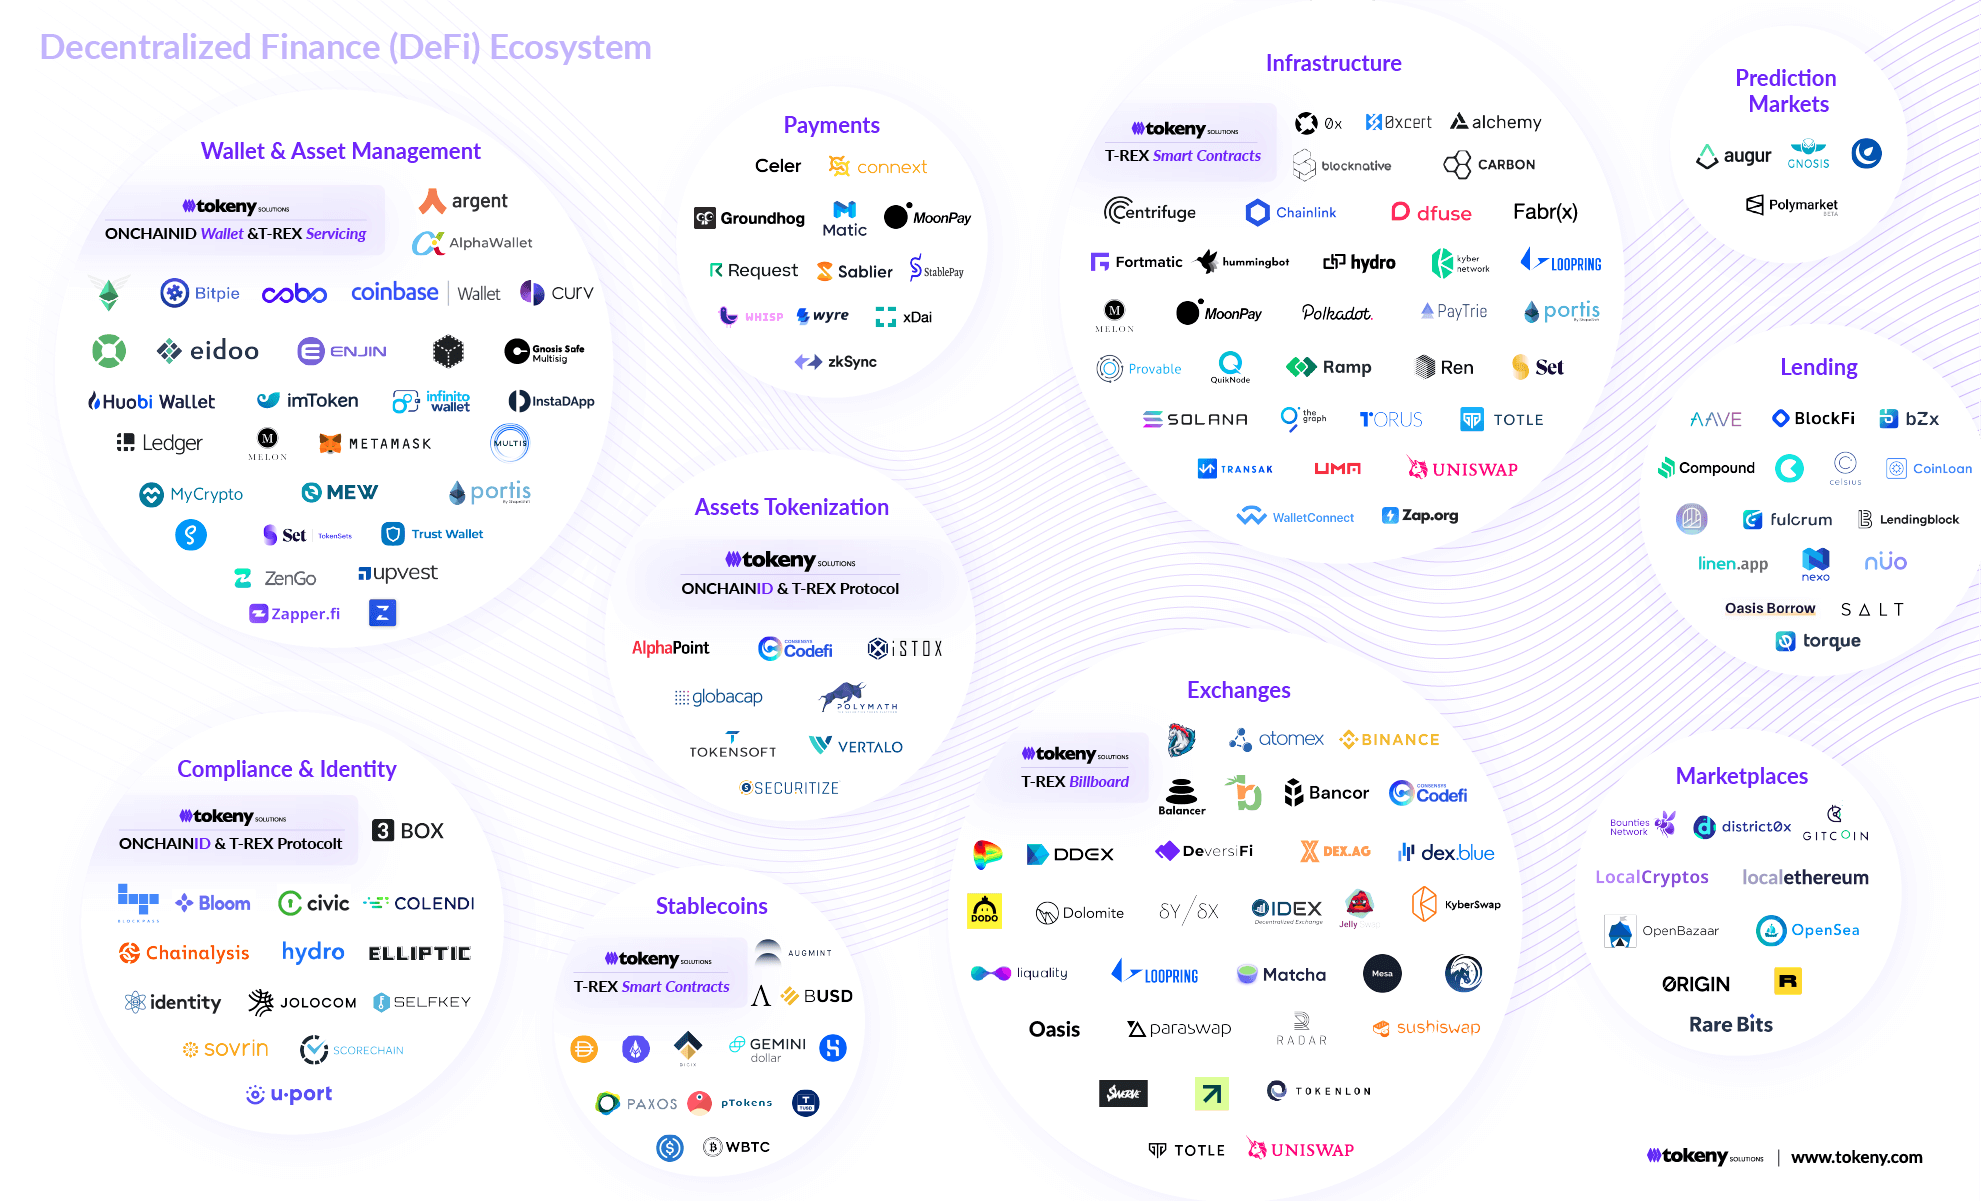
\includegraphics[width=0.8\linewidth]{DeFi-Ecosystem-Map.png}
    \caption{Экосистема DeFi}
    \label{fig:placeholder}
\end{figure}
\end{frame}

\subsection{DeFi vs TradFi}
\begin{frame}{DeFi vs TradFi}
  \setcounter{footnote}{0}
  \small
  \renewcommand{\arraystretch}{1.35}
  \begin{tabularx}{\textwidth}{@{}p{3cm}XX@{}}
    \toprule
    \textbf{Параметр} & \textbf{TradFi} & \textbf{DeFi} \\
    \midrule
    Доступ & Через посредника: KYC, счёт & Permissionless: кошелёк и интернет \\
    Расчёты & T+1 / T+2, часы работы биржи & Почти мгновенно, 24/7\footnotemark \\
    Кастодиан (депозитарий) & Банк / брокер держит актив & Self-custody или смарт-контракт \\
    Прозрачность & Баланс контрагента скрыт & Все транзакции видны ончейн\footnotemark \\
    Правила & Меняет оператор / регулятор & Заданы кодом --- пока не изменены governance\footnotemark \\
    \bottomrule
  \end{tabularx}
  \footnotetext[1]{Актуально прежде всего для трансграничных расчётов, а не для операций внутри одного банка или СБП}
  \footnotetext[2]{За исключением анонимизированных протоколов вроде \href{https://z.cash/}{ZCash}, \href{https://www.getmonero.org/}{Monero}}
  \footnotetext[3]{Governance-голосование может изменить параметры протокола}
\end{frame}

\begin{frame}{DeFi vs TradFi}
\begin{figure}
    \centering
    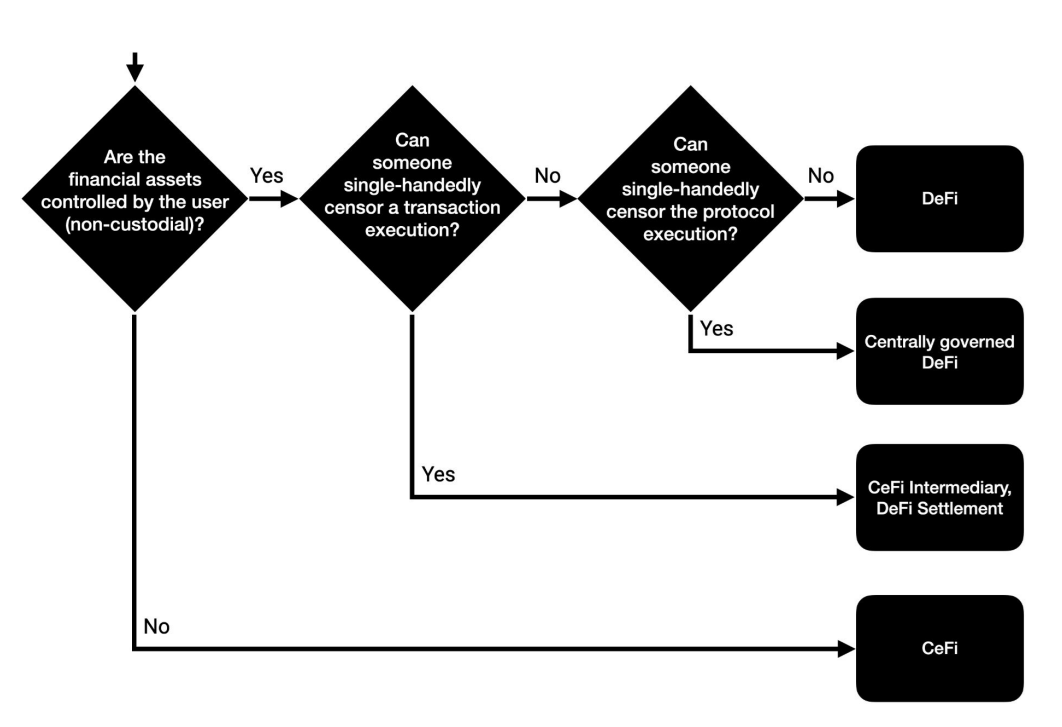
\includegraphics[width=0.48\linewidth]{cedefi.png}
    \caption{Это DeFi или нет?}
    \label{fig:cedefi}
\end{figure}
\footnotetext[5]{Из курса \href{https://rdi.berkeley.edu/berkeley-defi/f25}{Decentralized Finance}Fall 2025 University of Berkely}
\end{frame}

% ======================================================================
\section{Как устроен DeFi}
% ======================================================================

\subsection{Технологический фундамент}
\begin{frame}{Технологический фундамент}
  \begin{itemize}
    \item \textbf{Блокчейн} --- публичный реестр с детерминированным исполнением
    \begin{itemize}
      \item Общее состояние, которое все участники обновляют по одним правилам
    \end{itemize}
    % \vspace{-1mm}
    \centerline{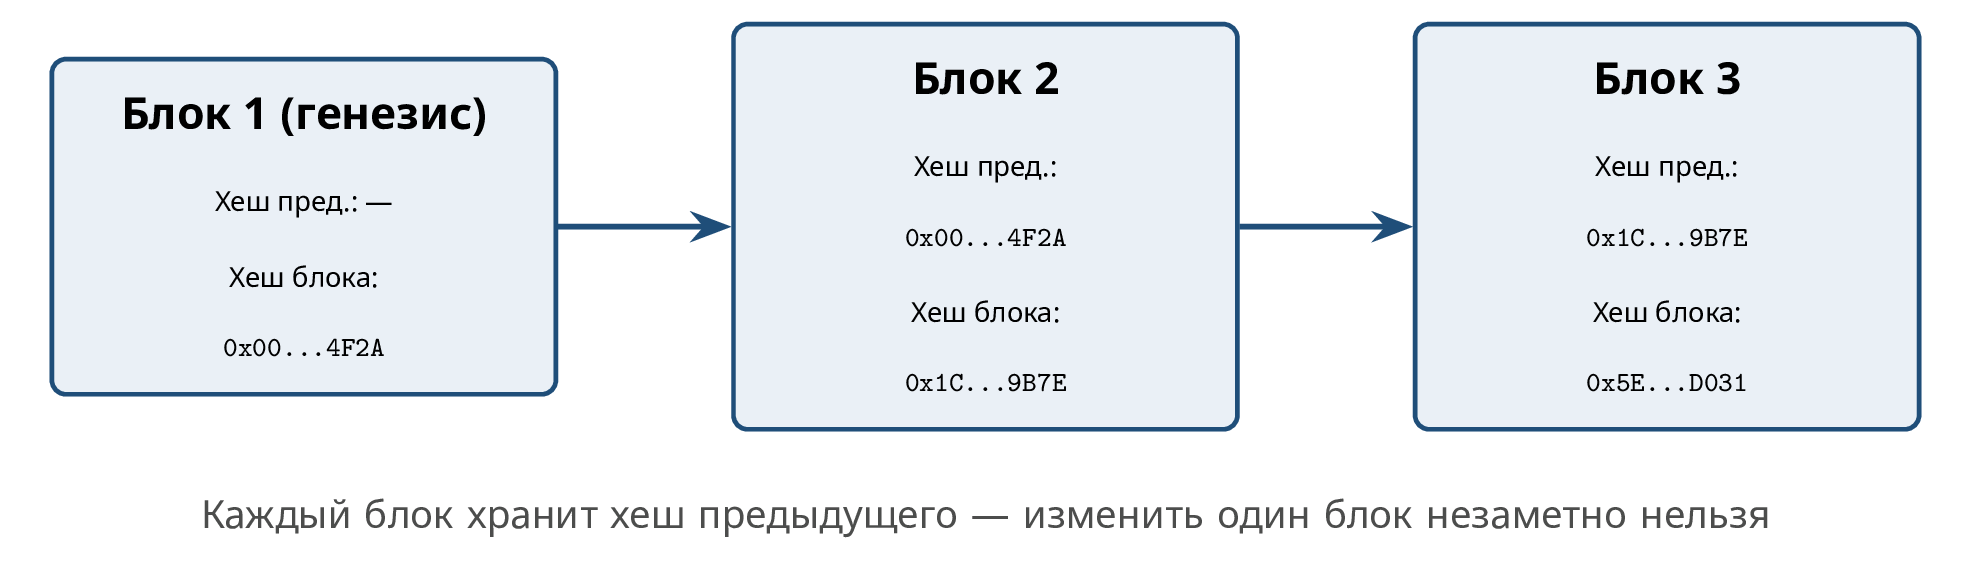
\includegraphics[width=0.58\textwidth]{blockchain.png}}
    \vspace{-2mm}
    \item \textbf{Смарт-контракт} --- код, который исполняется по заданным правилам. "вендинговый автомат"
    \begin{itemize}
      \item «Если X, то Y» --- прописано заранее и (обычно) неизменно
    \end{itemize}
    \item \textbf{Стейблкоин} --- мост между фиатным и ончейн миром
    \begin{itemize}
      \item Fiat-backed, crypto-backed, algorithmic --- отдельная большая тема \footnotemark
    \end{itemize}
  \end{itemize}

\footnotetext{ Чуть подробнее здесь: \href{https://docs.google.com/presentation/d/1X1zsJ3o4tnskKV3l7iiAg33HFhEAG335ropp0toxnHs/edit?usp=sharing}{Stablecoins} --- о дивный новый мир \textit{стабильности}}
\end{frame}

\subsection{Кошелёк и подпись транзакций}
\begin{frame}{Кошелёк --- точка входа в DeFi}
  \begin{columns}[T, onlytextwidth]
    \begin{column}{0.72\textwidth}
      \centering
      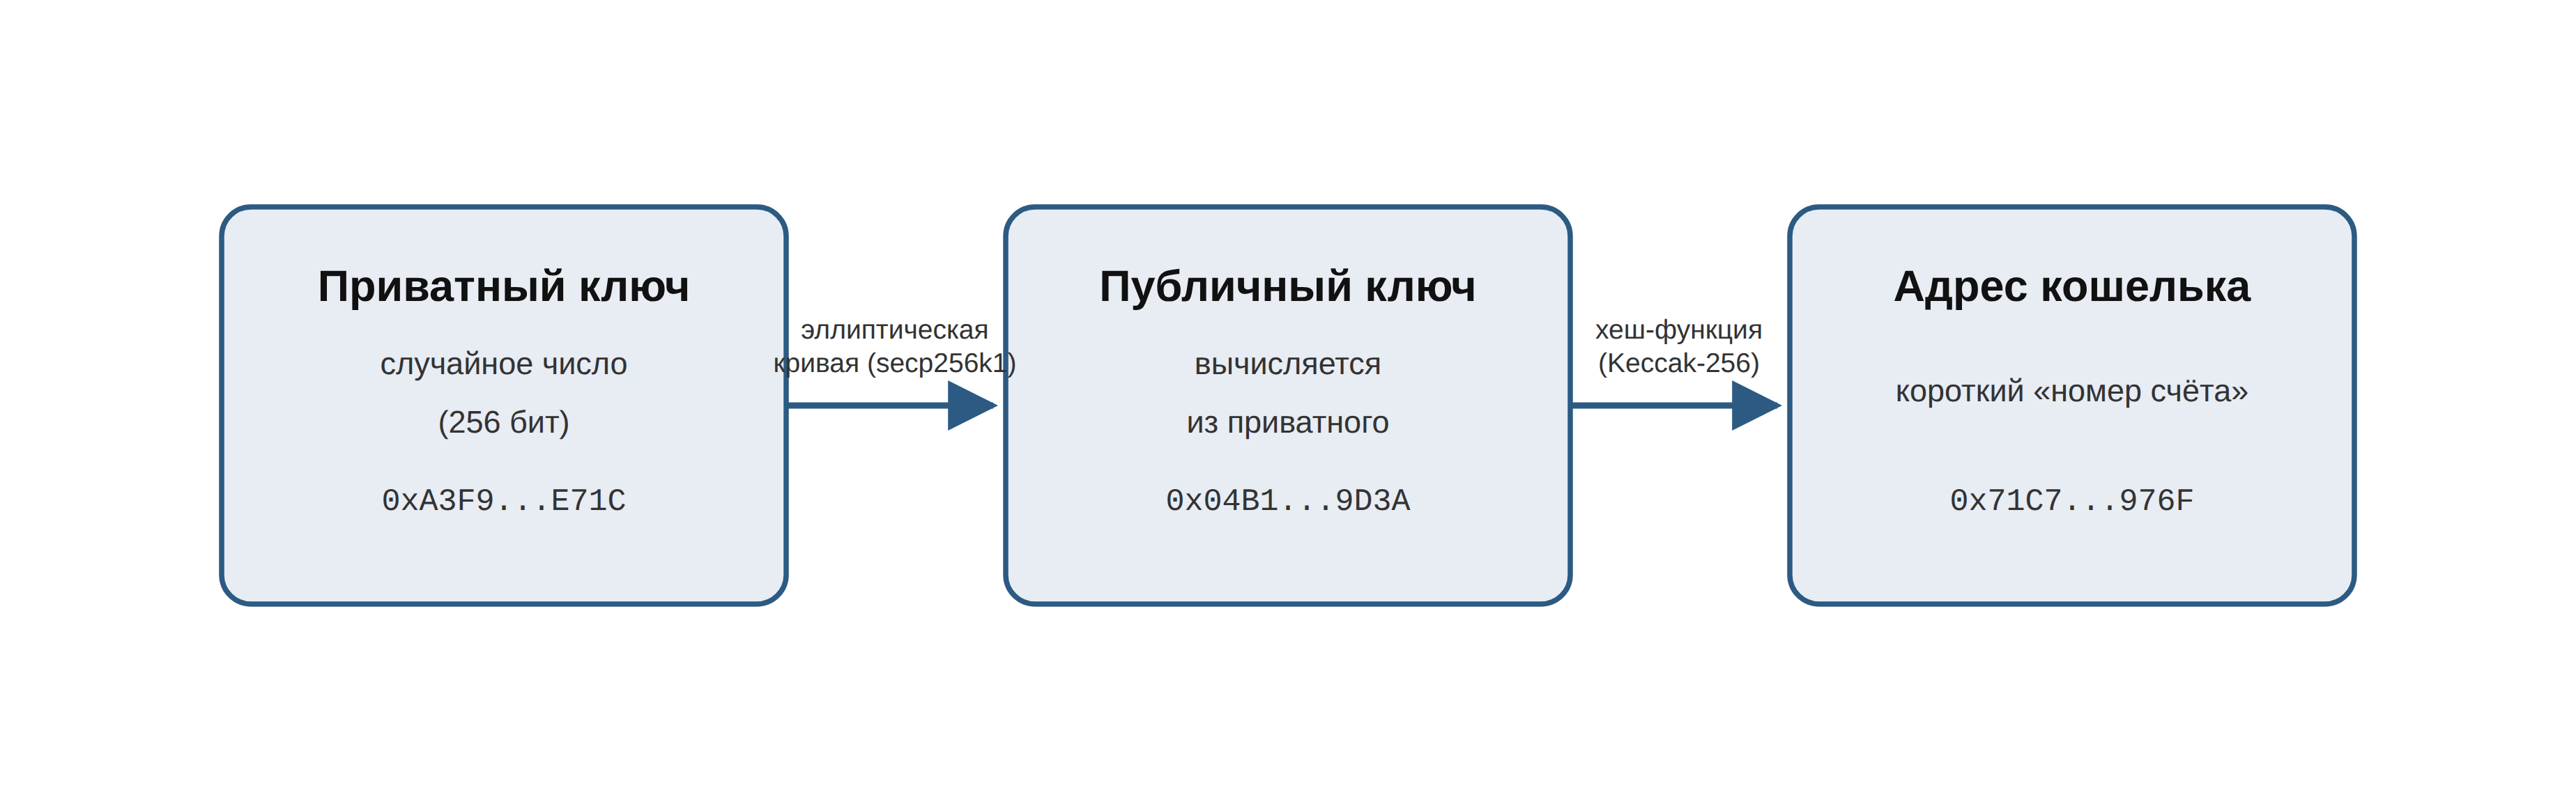
\includegraphics[width=\linewidth]{wallet-flow.png}
    \end{column}
    \begin{column}{0.24\textwidth}
      \centering
      \begin{tikzpicture}
        \node[draw=accent, thick, dash pattern=on 4pt off 3pt, inner sep=4pt] {
\includegraphics[width=0.9\linewidth]{qr.png}};
      \end{tikzpicture}
    \end{column}
  \end{columns}
  \vspace{1mm}
  \footnotesize
  \begin{block}{}
    \begin{itemize}
      \item Приватный ключ --- большое \textbf{случайное число}, единственное доказательство владения аккаунтом;
      \item Адрес --- производная от него, её можно свободно показывать.
      \item Подпись --- доказательство того, что именно вы отправили эту транзакция без раскрытия приватного ключа.
    \end{itemize}
\end{block}{}
\end{frame}

\subsection{Основные примитивы (money legos)}
\begin{frame}{Основные примитивы (money legos)}
  \small
  \renewcommand{\arraystretch}{1.32}
  \vfill
  \begin{tabularx}{\textwidth}{@{}*{3}{>{\raggedright\arraybackslash}p{2.7cm}}>{\raggedright\arraybackslash}X@{}}
    \toprule
    \textbf{Примитив} & \textbf{Примеры} & \textbf{TradFi-аналог} & \textbf{Что решает} \\
    \midrule
    Стейблкоины & USDC, DAI & Фиатные деньги & Единица расчётов ончейн \\
    DEX / AMM & Uniswap, Curve & Маркетмейкинг & Обмен активов без ордербука и брокера \\
    Lending / Borrowing & Aave, Compound & Money market, репо & Кредит под залог без банка и кредитной истории \\
    Деривативы / перпетуалы & dYdX, GMX & Фьючерсы, свопы & Деривативы без центрального клиринга \\
    Staking / Liquid staking & Lido, Rocket Pool & Срочный депозит & Доход за участие в безопасности сети \\
    \bottomrule
  \end{tabularx}
  \vfill
\end{frame}

\subsection{DEX и AMM: как происходит своп}
\begin{frame}{DEX и AMM: как происходит своп (обмен токенами)}
  \vspace{-3mm}
  \begin{columns}[b, onlytextwidth]
    \begin{column}{0.48\textwidth}
      \begin{figure}
        \centering
        \begin{minipage}[b][5cm][c]{\linewidth}
          \centering
          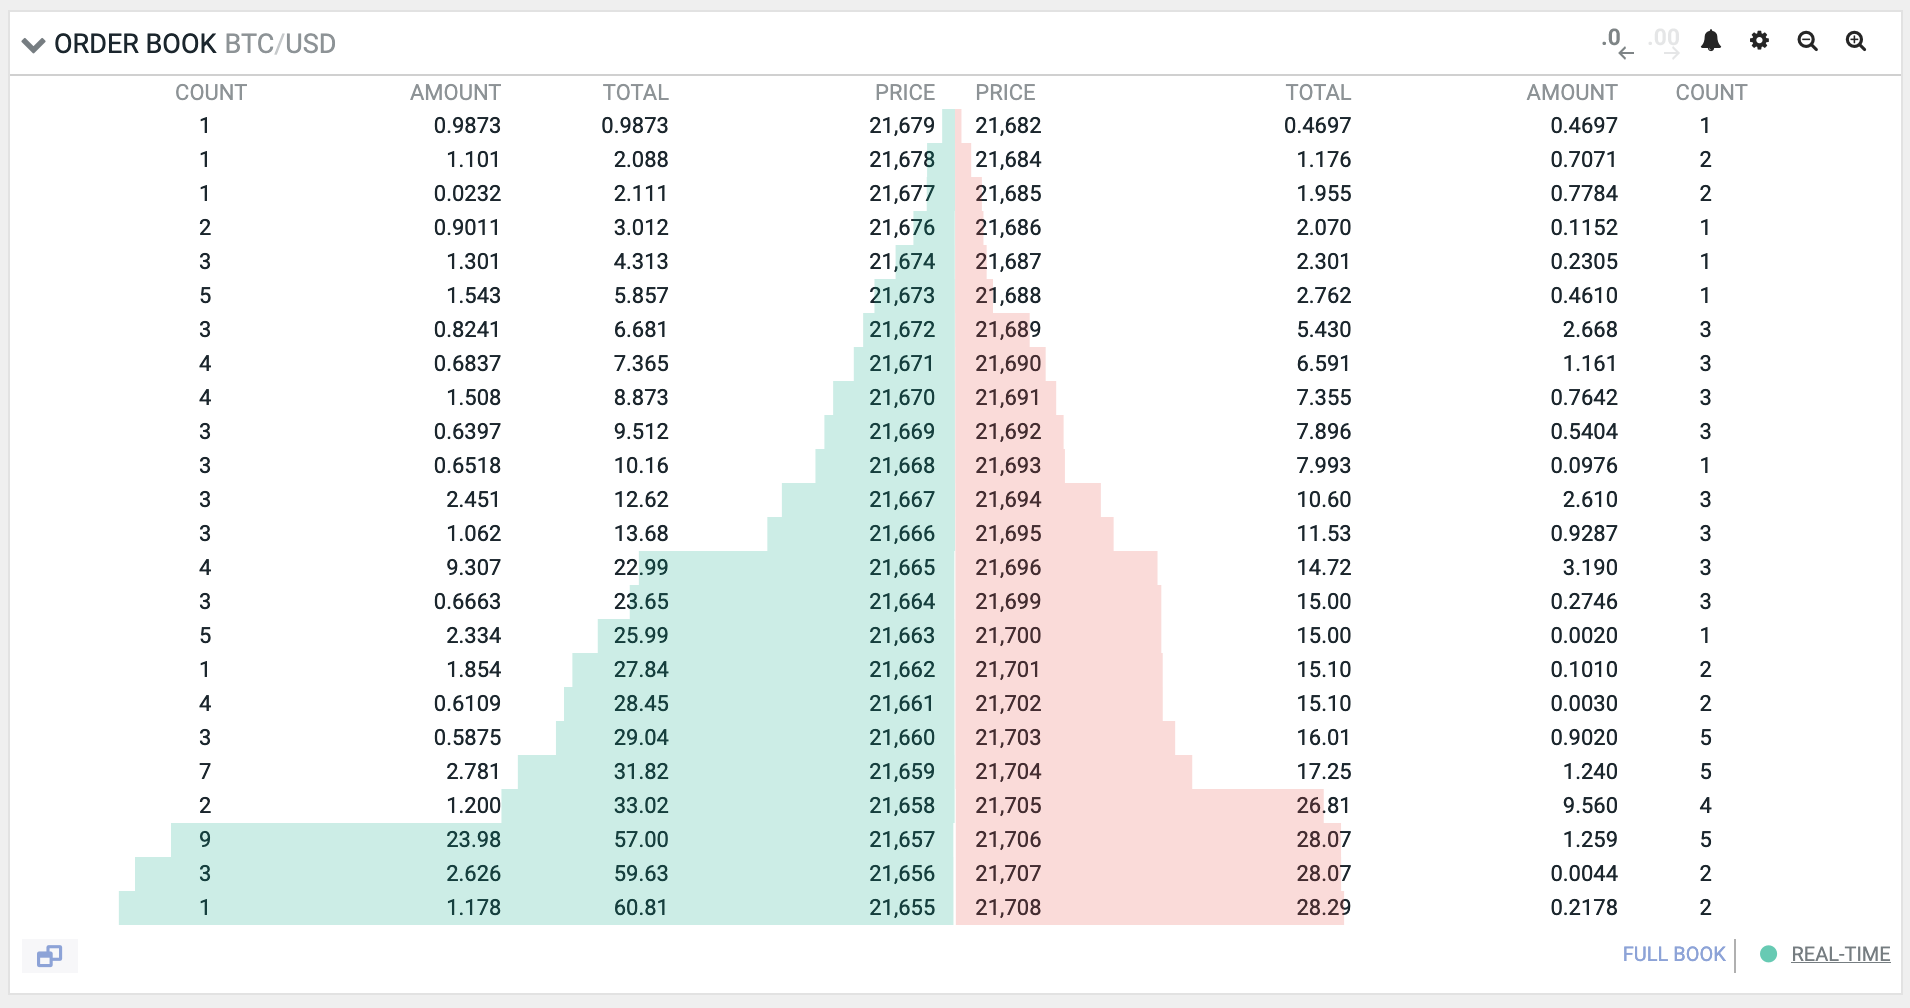
\includegraphics[width=\linewidth, height=5cm, keepaspectratio]{orderbook.png}
        \end{minipage}
        \caption{Ордербук}
        \label{fig:orderbook}
      \end{figure}
    \end{column}
    \begin{column}{0.48\textwidth}
      \begin{figure}
        \centering
        \begin{minipage}[b][5cm][c]{\linewidth}
          \centering
          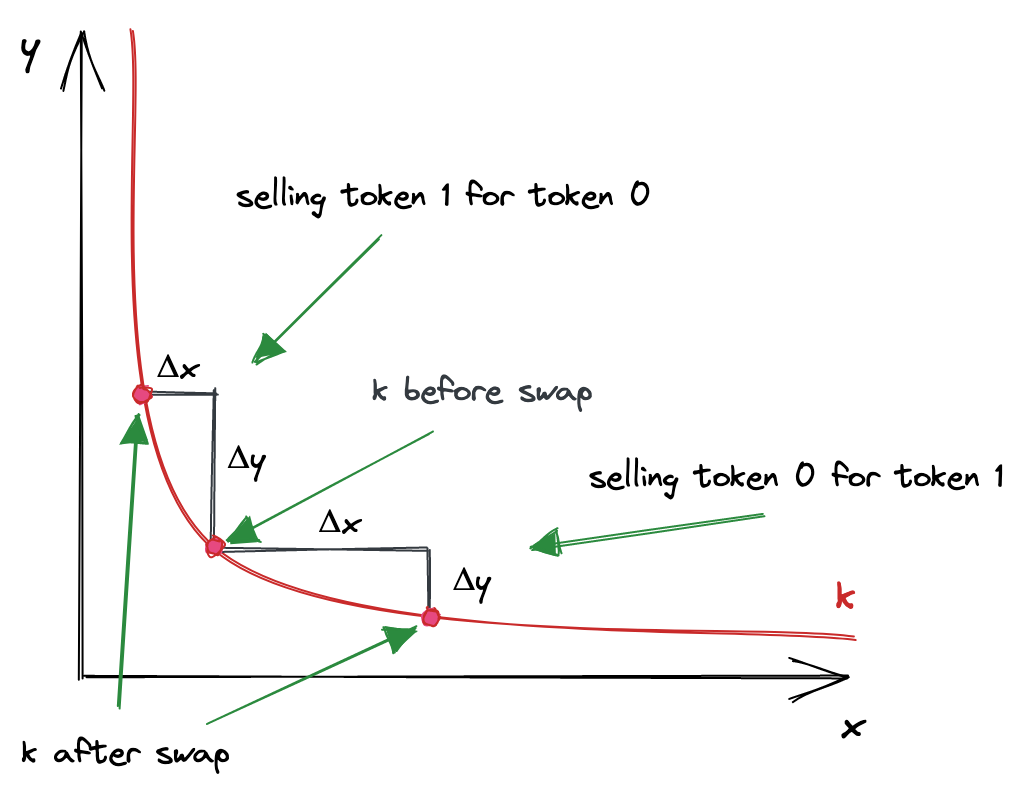
\includegraphics[width=\linewidth, height=5cm, keepaspectratio]{the_curve.png}
        \end{minipage}
        \caption{AMM}
        \label{fig:amm-curve}
      \end{figure}
    \end{column}
  \end{columns}
\end{frame}

\begin{frame}{DEX и AMM: как происходит своп (обмен токенами)}
  \begin{block}{Как AMM определяет цену}
    \footnotesize
    \setlength{\itemsep}{0pt}
    \setlength{\topsep}{0pt}
    \setlength{\parskip}{0pt}
    \begin{itemize}
      \item Ордербук: покупатели и продавцы выставляют встречные заявки (bid-ask), цена сделки --- точка их пересечения;
      \item AMM: ликвидность лежит в общем пуле (от Liquidity Providers), цена --- функция его состава (пропорции токенов), а не заявок отдельных участников рынка;
      \item Самый распространённый инвариант --- \textbf{constant product}: $x \cdot y = k$, где $x, y$ --- запасы двух токенов в пуле;
      \item Своп меняет величины $x$ и $y$, но не величину $k$ --- отсюда проскальзывание (slippage) на крупных сделках и impermanent loss для LP. Функции прироста $\Delta x$ и $\Delta y$ нелинейны!
    \end{itemize}
  \end{block}
\end{frame}


\subsection{Lending: обеспечение и ликвидация}
\begin{frame}{Lending: обеспечение и ликвидация}
  \vspace{1mm}
  \centering
  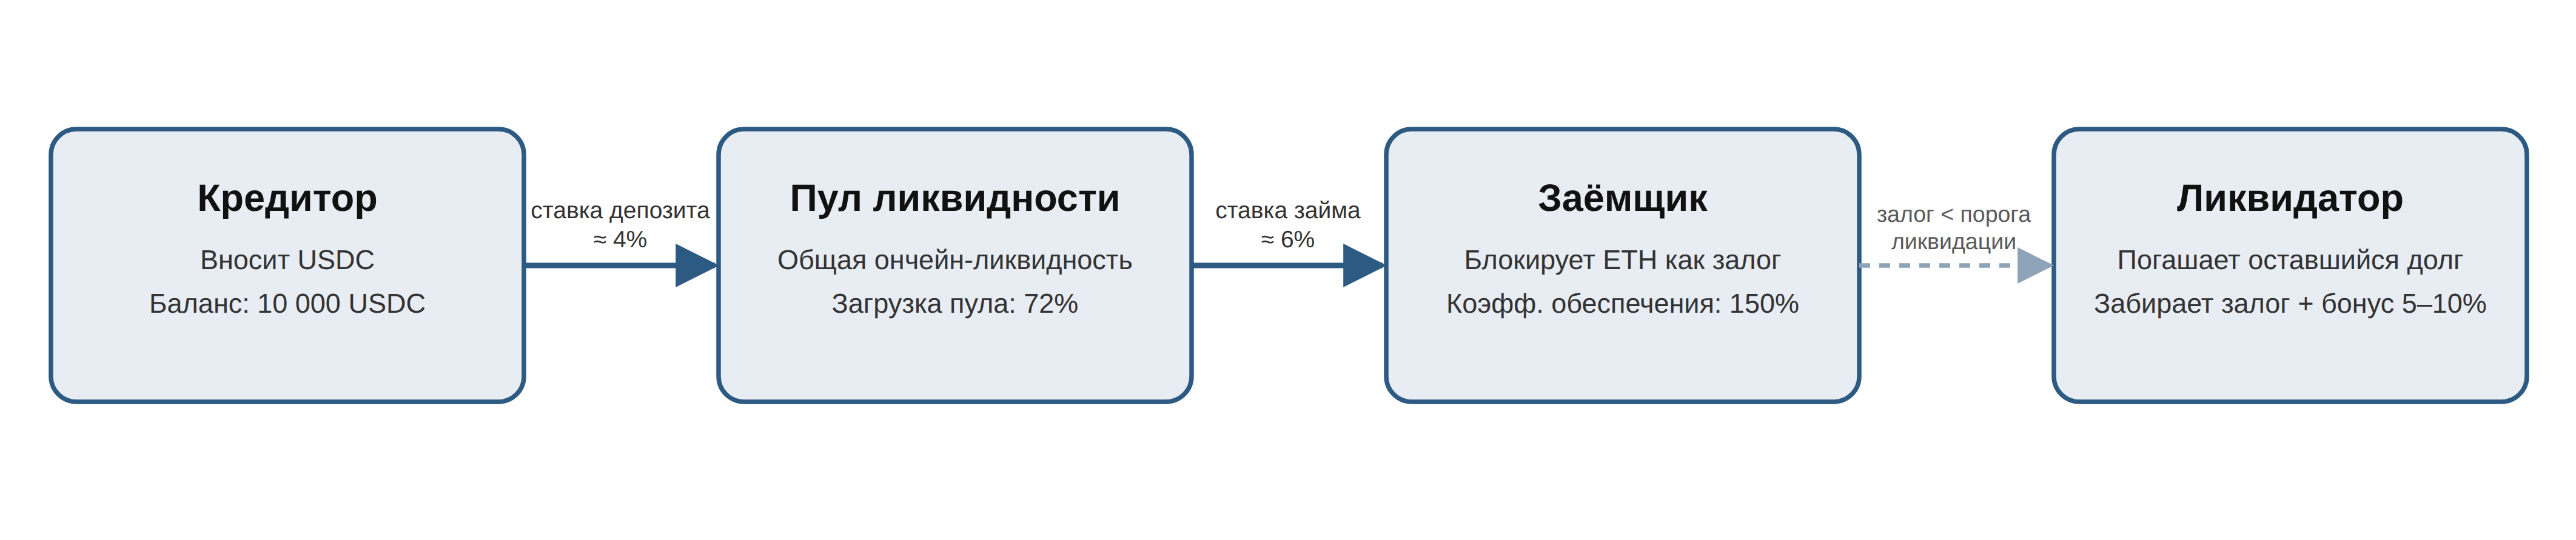
\includegraphics[width=\linewidth]{lending_diagram.png}
  \begin{block}{Как это работает}
    \small
    \begin{itemize}
      \item Обеспечение почти всегда избыточно (over-collateralized), так как это единственная защита протокола от дефолта без кредитной истории заёмщика.
      \item Если стоимость залога падает ниже порога (liquidation ratio), ликвидаторы гасят долг и забирают залог с дисконтом --- риск каскадного эффекта при резком падении рынка.
    \end{itemize}
  \end{block}
\end{frame}

\begin{frame}{Lending: рост рынка}
  \centering
  \begin{figure}
    \centering
    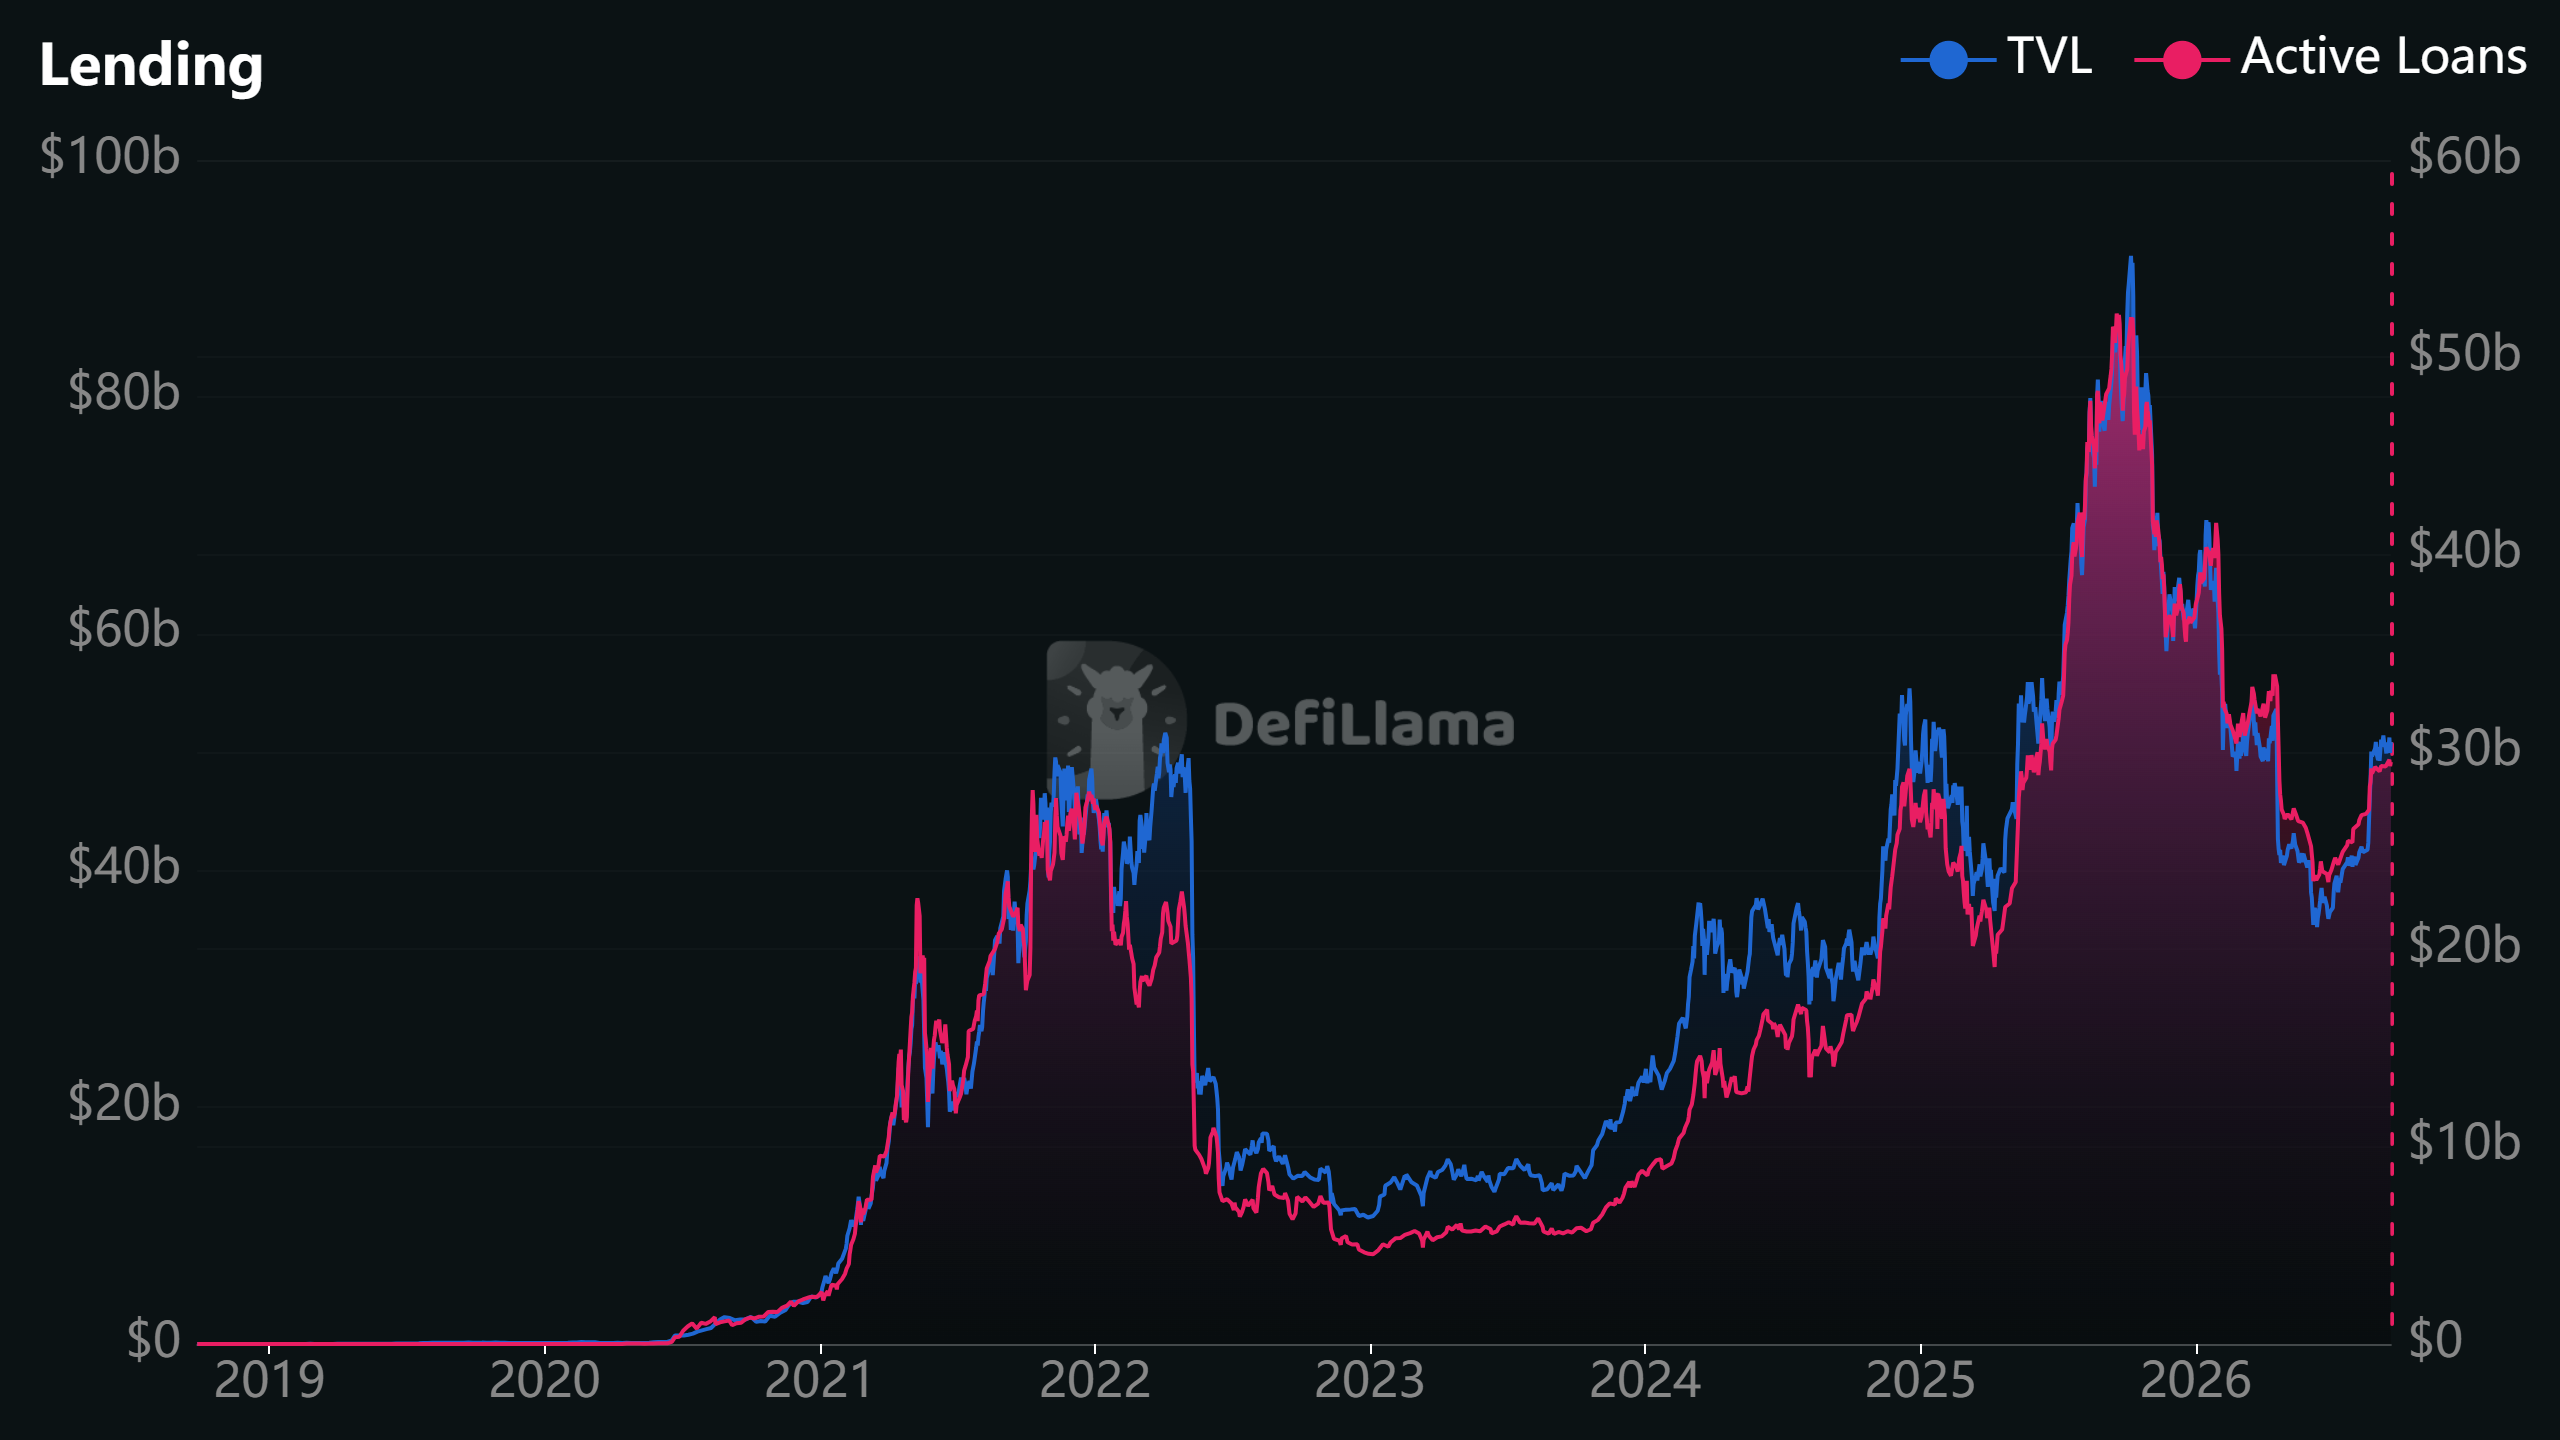
\includegraphics[width=0.62\linewidth]{tvl_loans.png}
    \caption{TVL и объём активных займов в lending-протоколах}
    \label{fig:tvl-loans}
  \end{figure}
\end{frame}

\subsection{Инфраструктура: оракулы, мосты, L1/L2}
\begin{frame}{Элементы инфраструктуры: оракулы}
  \vspace{1mm}
  \centering
  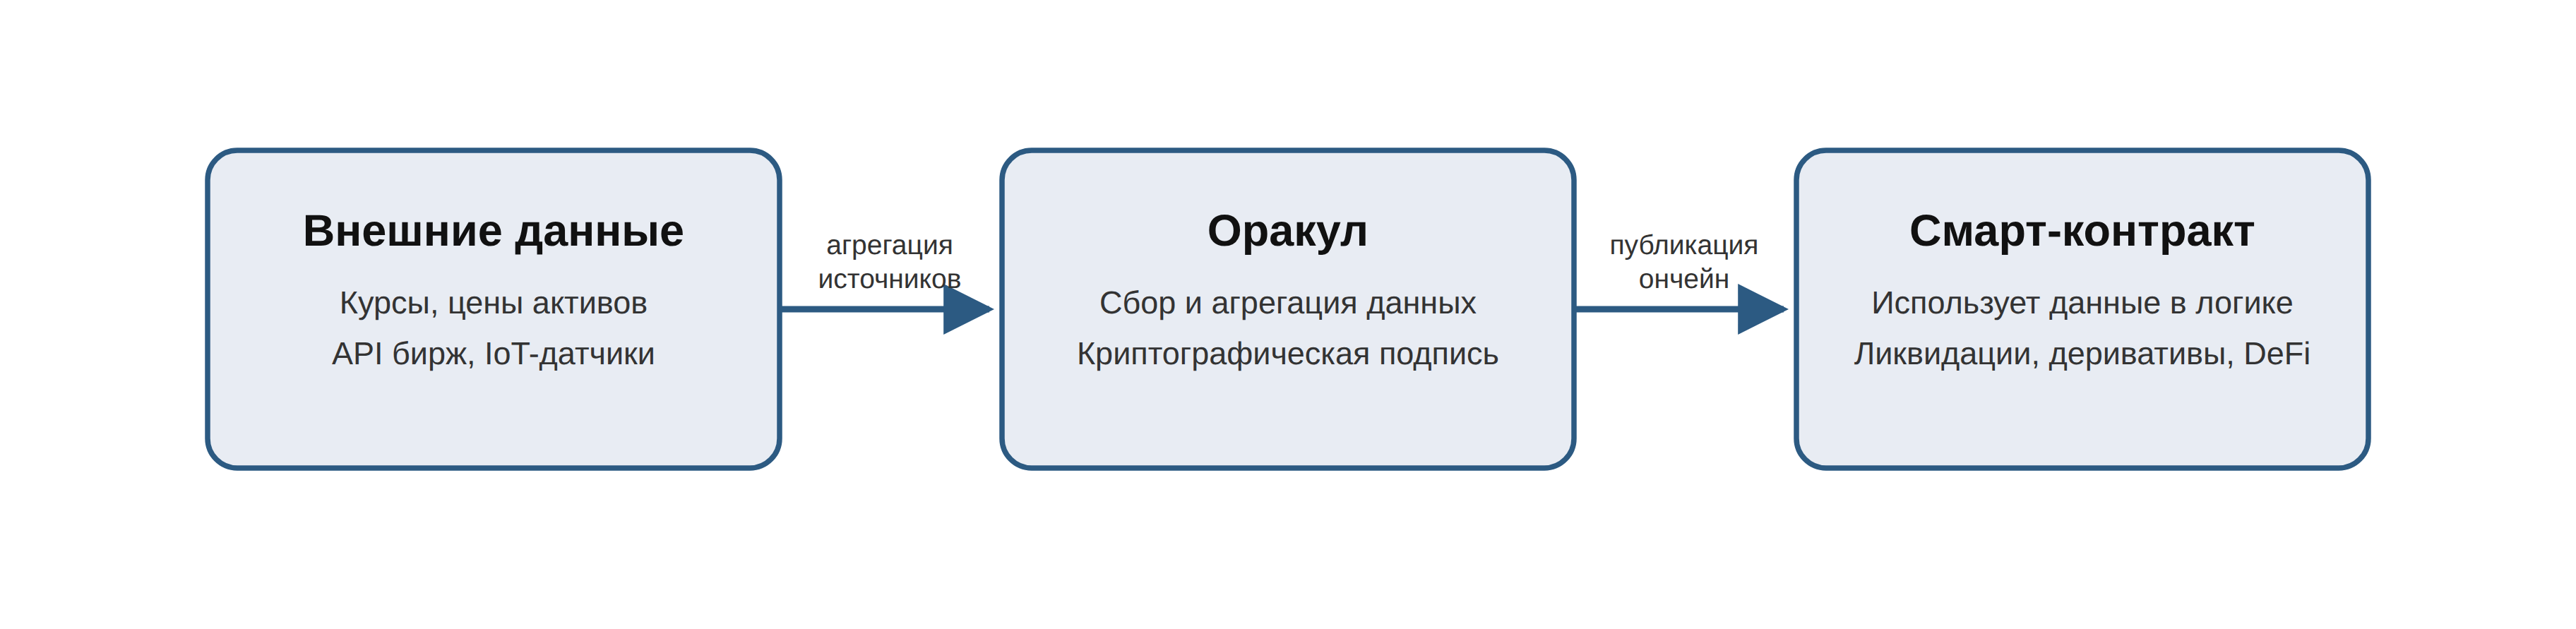
\includegraphics[width=\linewidth]{oracles_diagram.png}
  \begin{block}{Оракулы (Chainlink и др.)}
    \small
    \begin{itemize}
      \item Поставляют данные из внешнего мира (цены, курсы) в смарт-контракт.
      \item Блокчейн --- детерминированная среда: каждый валидатор должен получить одинаковый результат, поэтому напрямую обращаться в интернет он не может --- данные там могут измениться.
    \end{itemize}
  \end{block}
\end{frame}

\begin{frame}{Элементы инфраструктуры: мосты}
  \vspace{1mm}
  \centering
  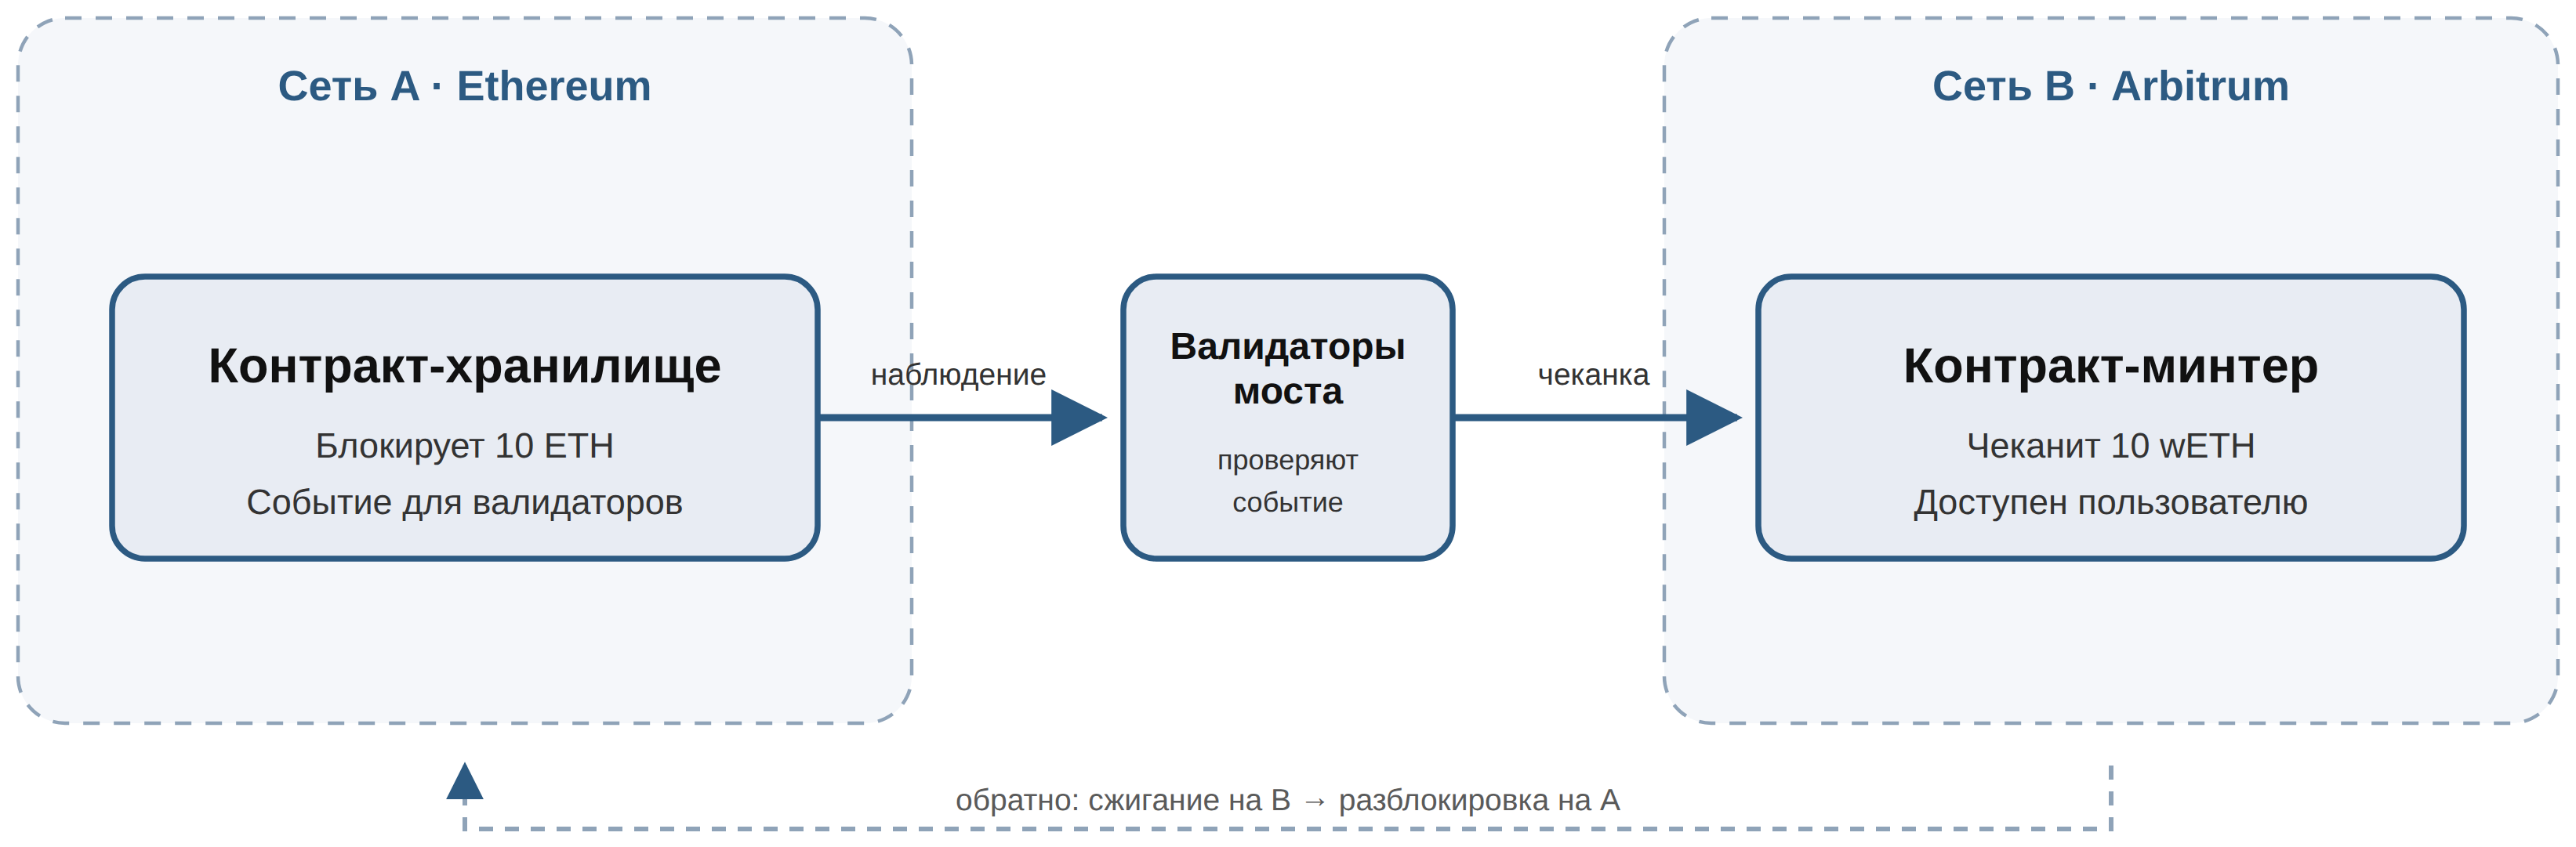
\includegraphics[width=\linewidth]{bridges_diagram.png}
  \begin{block}{Мосты (bridges)}
    \small
    \begin{itemize}
      \item Нужны для переноса активов из одной сети в другую
      \item Одна из самых частых точек взлома в DeFi
    \end{itemize}
  \end{block}
\end{frame}

\begin{frame}{Элементы инфраструктуры: L1/L2}
  \vspace{1mm}
  \centering
  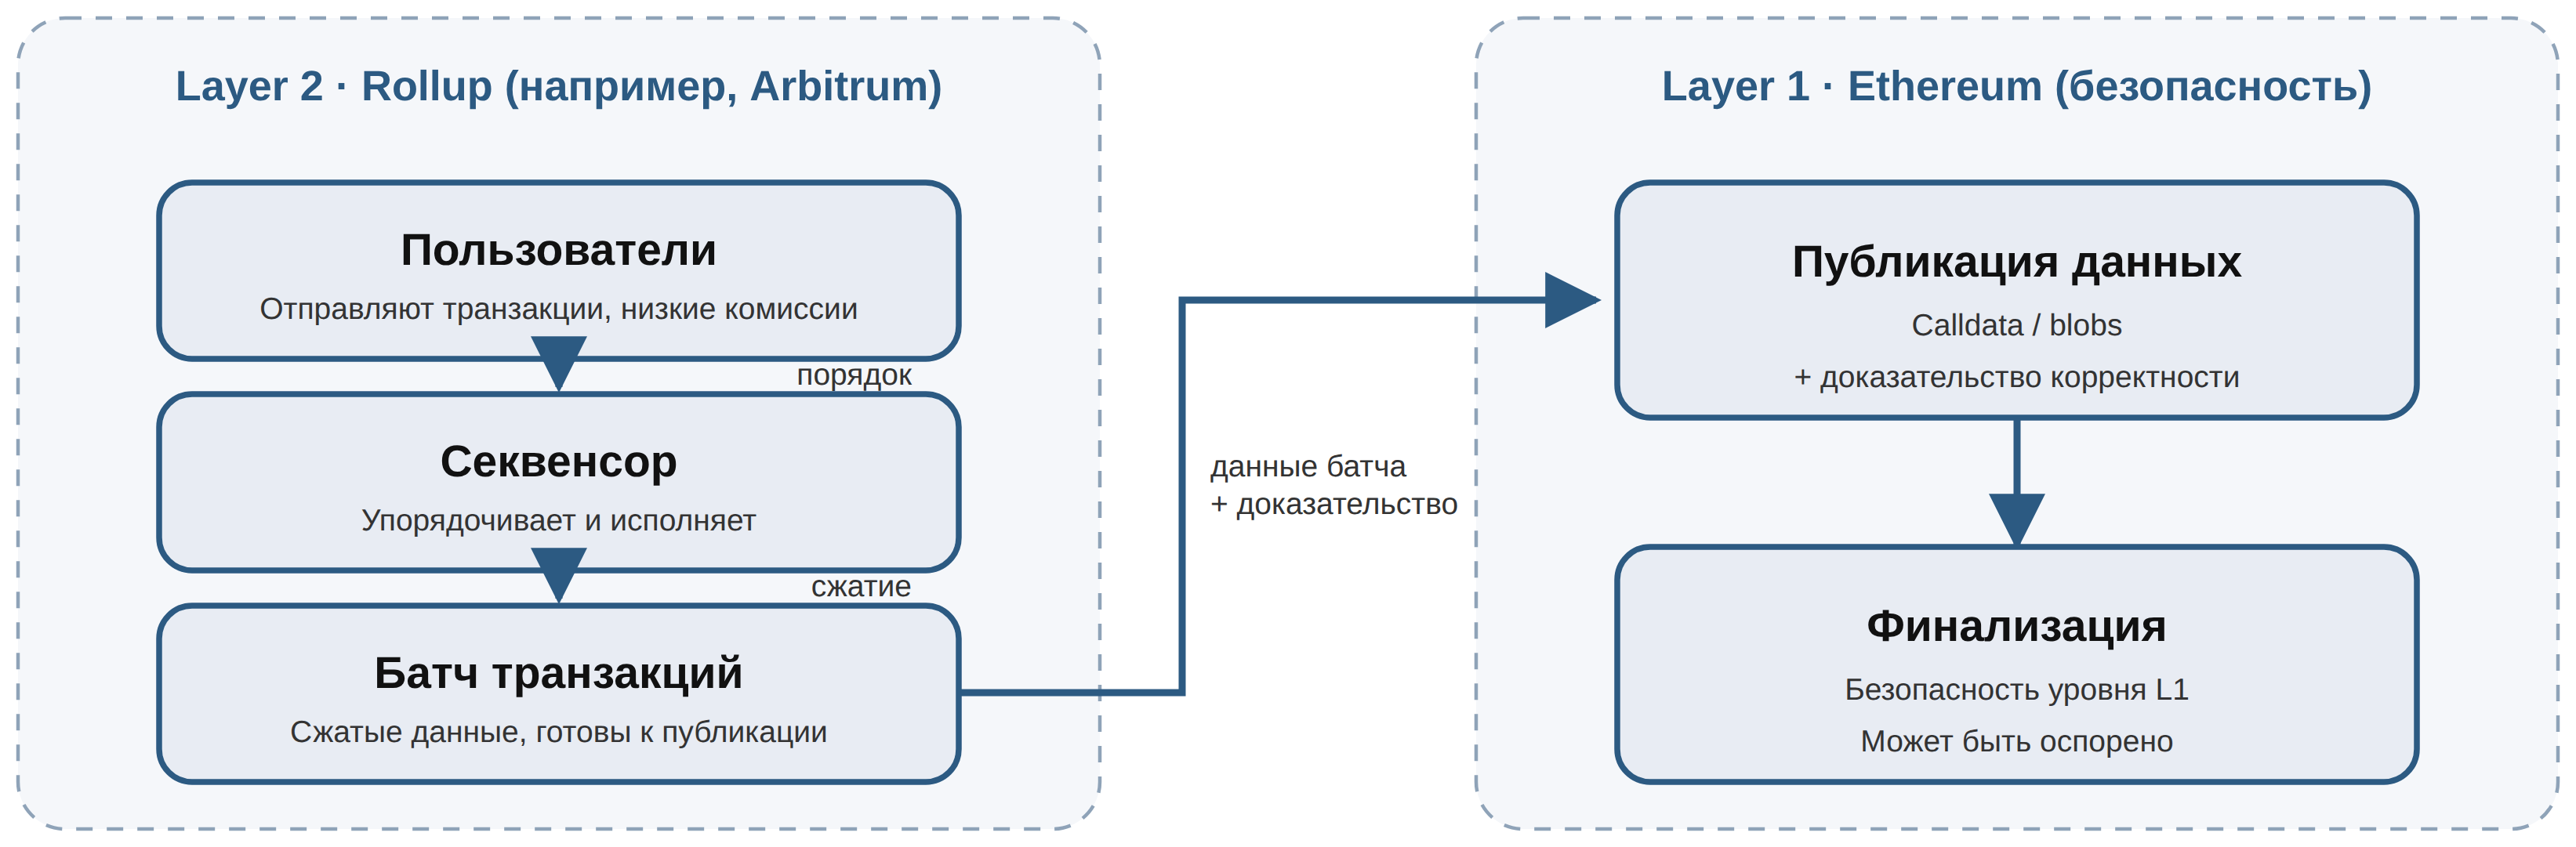
\includegraphics[width=\linewidth]{l2_diagram.png}
  \begin{block}{L1 / L2}
    \small
    \begin{itemize}
      \item Базовый блокчейн и надстройки над ним для масштабирования
      \item Trade-off: децентрализация против скорости и стоимости транзакций
    \end{itemize}
  \end{block}
\end{frame}

% ======================================================================
\section{Риски и что дальше}
% ======================================================================

\subsection{Карта рисков}
\begin{frame}{Карта рисков DeFi}
  \centering
  \begin{figure}
    \centering
    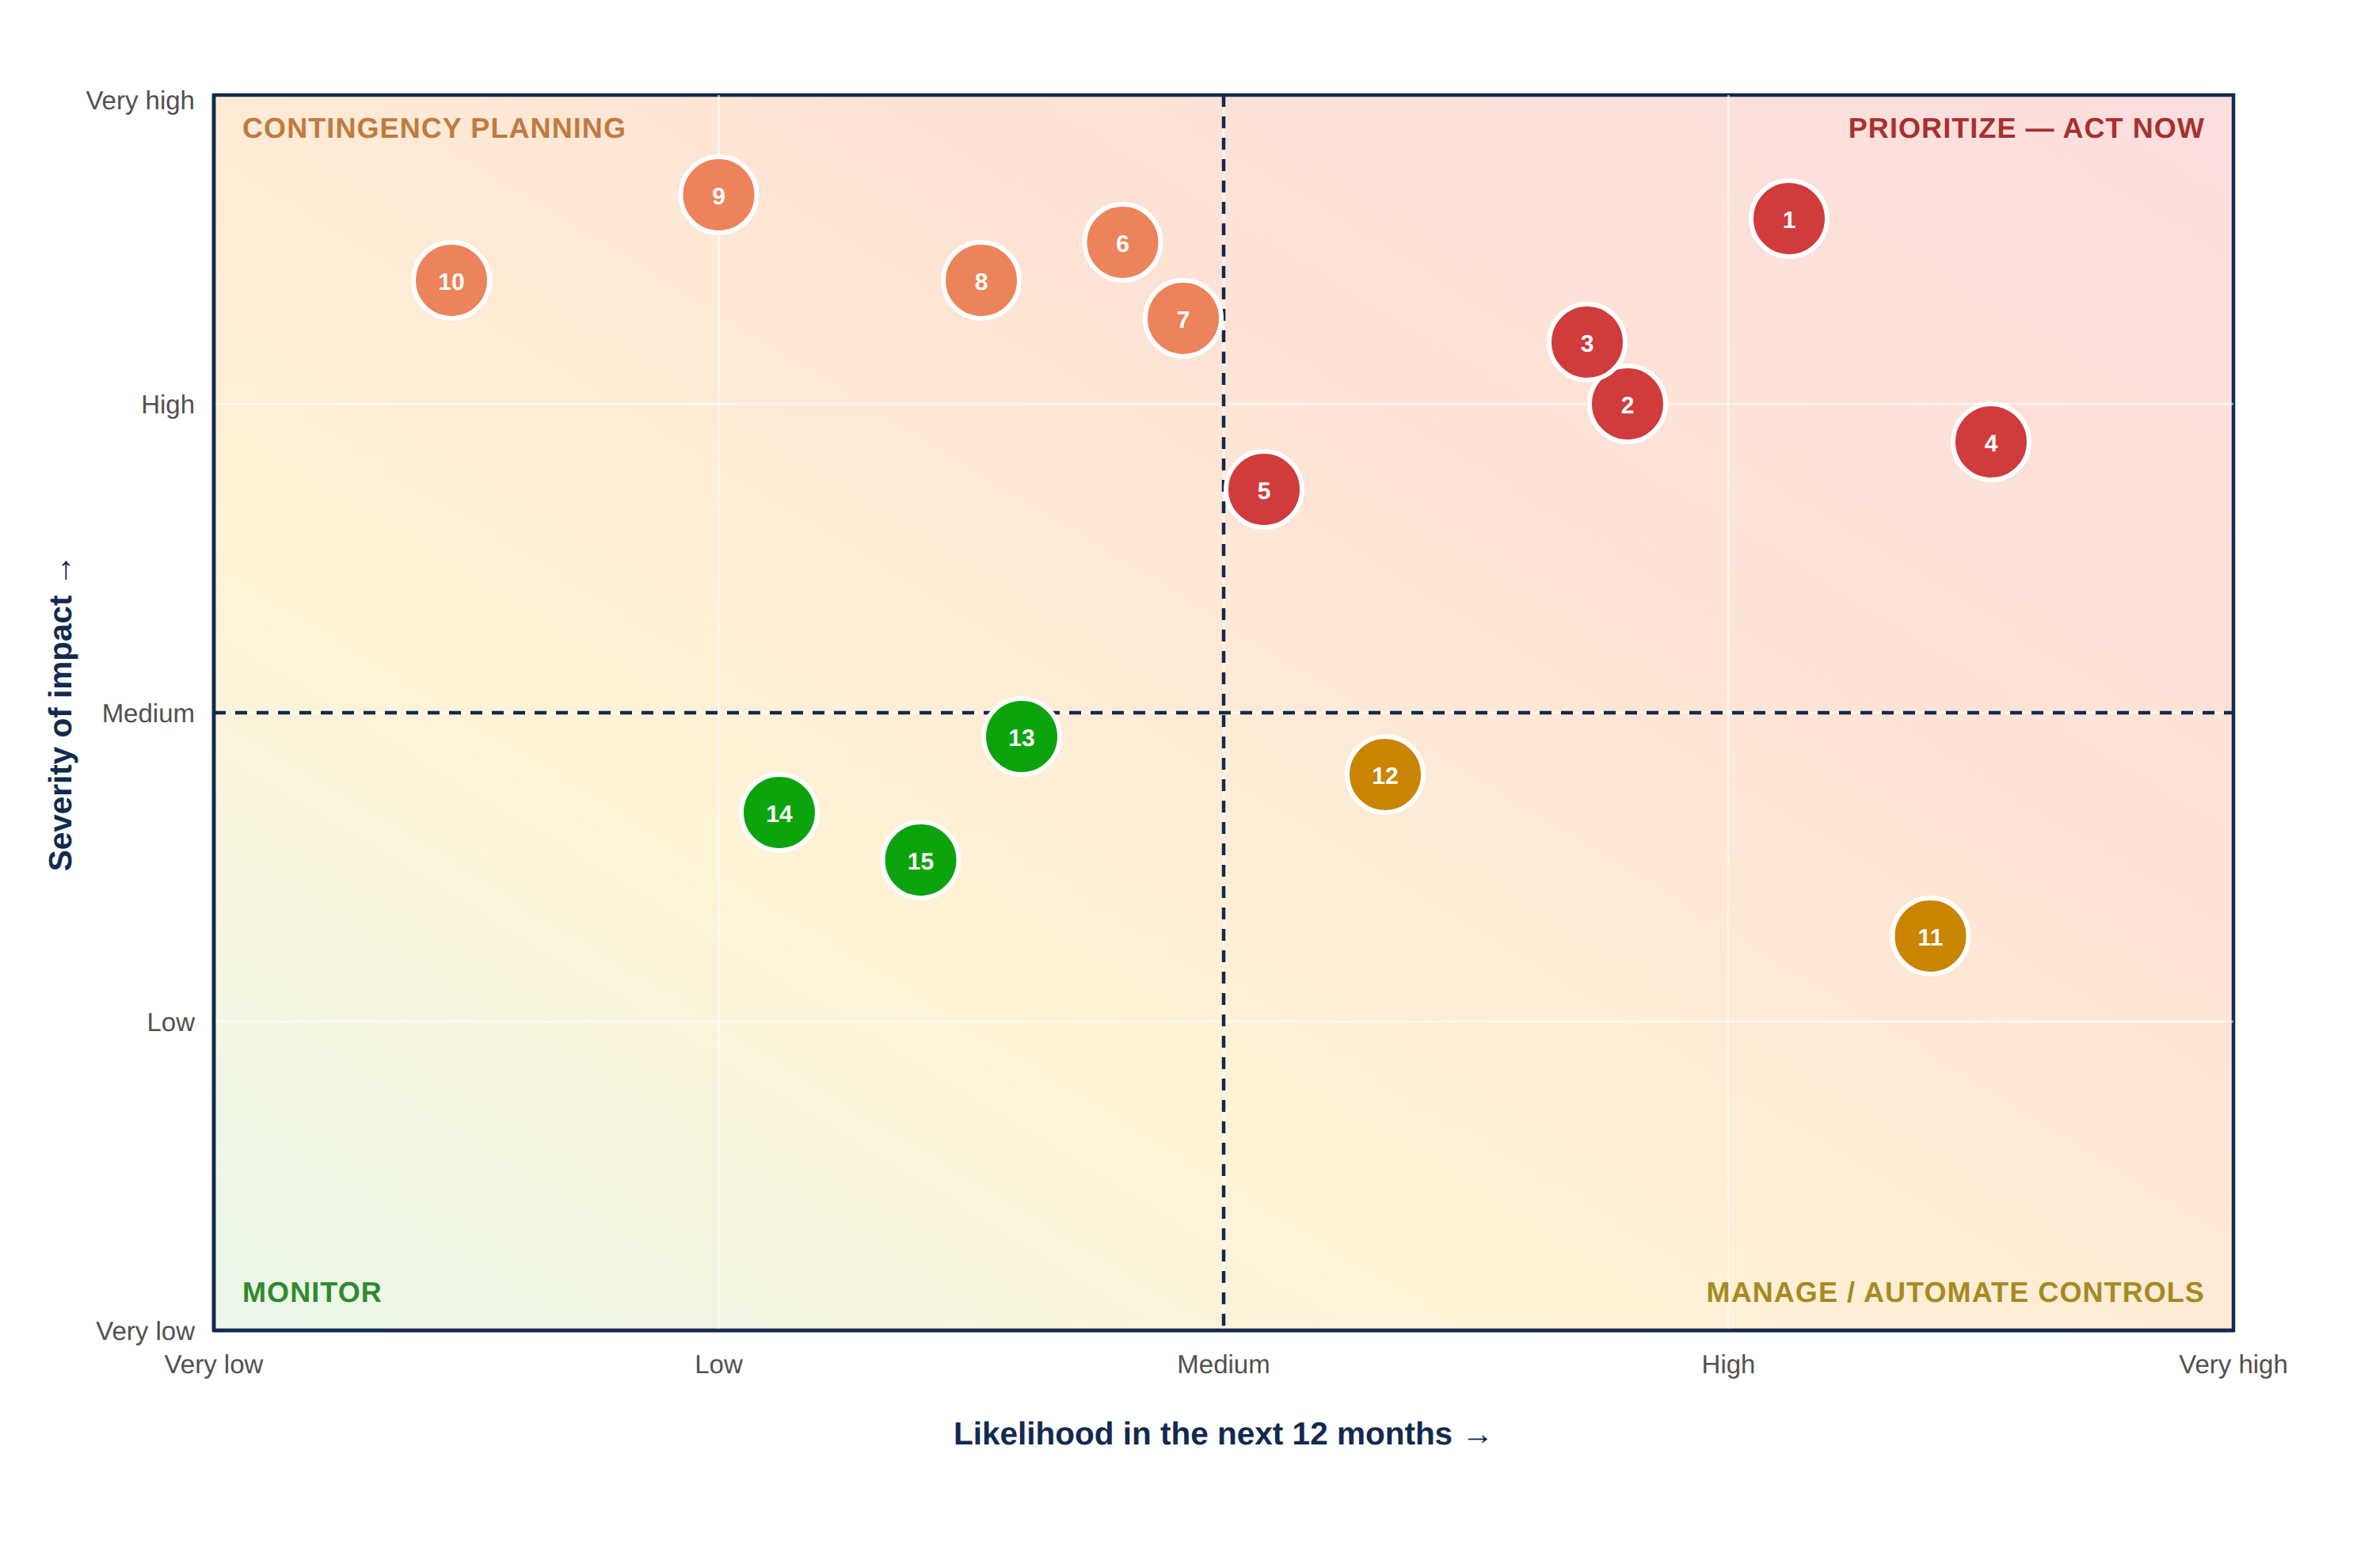
\includegraphics[width=0.56\linewidth]{defi_risk_matrix_only.png}
    \caption{Вероятность реализации риска (12 мес) и тяжесть последствий}
    \label{fig:risk-matrix}
  \end{figure}
\end{frame}

\begin{frame}{Карта рисков DeFi: ключевые риски}
  \footnotesize
  \begin{columns}[T, onlytextwidth]
    \begin{column}{0.5\textwidth}
      \begin{block}{Приоритет --- действовать}
        \begin{enumerate}
          \setlength{\itemsep}{0pt}
          \item Смарт-контракты: баги, эксплойты
          \item Манипуляция оракулами
          \item Каскады ликвидаций (плечо)
          \item Регуляторные шоки
          \item Рестейкинг / re-hypothecation
        \end{enumerate}
      \end{block}
      \vspace{2mm}
      \begin{block}{Контроль / автоматизация}
        \begin{enumerate}
          \setlength{\itemsep}{0pt}
          \setcounter{enumi}{10}
          \item MEV и сэндвич-атаки
          \item RWA: юридические и кастодиальные пробелы
        \end{enumerate}
      \end{block}
    \end{column}
    \begin{column}{0.5\textwidth}
      \begin{block}{План B --- ниже вероятность}
        \begin{enumerate}
          \setlength{\itemsep}{0pt}
          \setcounter{enumi}{5}
          \item Эксплойты кросс-чейн мостов
          \item Компрометация admin-key / мультисига
          \item Депег стейблкоинов
          \item Каскад CeFi--DeFi
          \item Квантовая угроза для ECDSA-подписей
        \end{enumerate}
      \end{block}
      \vspace{2mm}
      \begin{block}{Мониторинг}
        \begin{enumerate}
          \setlength{\itemsep}{0pt}
          \setcounter{enumi}{12}
          \item Недокапитализация страхового фонда
          \item Governance-атака через флэш-займы
          \item Централизация L2-секвенсера
        \end{enumerate}
      \end{block}
    \end{column}
  \end{columns}
\end{frame}

\subsection{Регулирование в РФ}
\begin{frame}{282-ФЗ}
  По определению и по архитектуре на сам DeFi невозможно оказать влияние. Однако можно зарегулировать посредников и пути доступа к протоколам DeFi.
  \begin{itemize}
    \item Лицензируются биржи, обменники, депозитарии;
    \item Цифровая валюта признаётся имуществом;
    \item Некастодиальные кошельки и cooling-off период в 48 часов при переводе более 100 000 руб.
    \item Расчёты криптовалютой внутри России по-прежнему запрещены, но участникам ВЭД разрешены трансграничные расчёты и переводы криптовалюты за рубеж
  \end{itemize}
\end{frame}

% ------------------------------------------------------------- sources ---
\begin{frame}{Источники}
  \small
  \begin{enumerate}
    \item Uniswap v2 Core --- whitepaper
    \item Aave Protocol --- документация
    \item Chainlink Docs --- оракулы
    \item DeFiLlama --- данные по TVL и протоколам
    \item BIS --- обзоры о DeFi и системных рисках
    \item EUR-Lex --- регламент MiCA (EU)
  \end{enumerate}
\end{frame}

\end{document}